\documentclass[conference]{IEEEtran}
%	\IEEEoverridecommandlockouts
\usepackage{cite}
\usepackage{amsmath,amssymb,amsfonts}
%	\usepackage{algorithmic}
\usepackage[dvipdfmx]{graphicx}
\usepackage{graphicx}
\usepackage{color}
\usepackage{textcomp}
\usepackage{xcolor}
\definecolor{blue}{rgb}{0.00, 0.00, 1.00}
\usepackage{listings}
\usepackage{datetime2}
\usepackage{algorithm}
\usepackage{algorithmicx}
\usepackage{algpseudocode}
%	\usepackage{comment}
\def\BibTeX{{\rm B\kern-.05em{\sc i\kern-.025em b}\kern-.08em T\kern-.1667em\lower.7ex\hbox{E}\kern-.125emX}}
\lstset{
  language={Fortran},
  basicstyle={\ttfamily},
  identifierstyle={\small},
  %	commentstyle={\smallitshape},
  % keywordstyle={\small\bfseries},
  keywordstyle={\small},
  ndkeywordstyle={\small},
  %	stringstyle={\small\ttfamily},
  frame={tb},
  breaklines=true,
  columns=[l]{fullflexible},
  numbers=left,
  xrightmargin=0zw,
  xleftmargin=2zw,
  numberstyle={\scriptsize},
  stepnumber=1,
  numbersep=1zw,
  lineskip=-0.5ex,
  %	belowcaptionskip=10pt,abovecaptionskip=10pt
}


\begin{document}

\title{
%
%	\textcolor{blue}{as of \DTMnow} \\
%
Performance evaluation and visualization of scientific applications using PMlib
}

% double blinded proof reading version
% \if 0
\author{
\IEEEauthorblockN{1\textsuperscript{st} Kazunori Mikami}
\IEEEauthorblockA{\textit{Flagship 2020 Project} \\
\textit{Riken R-CCS}\\
Kobe, Japan \\
kazunori.mikami@riken.jp}
\and
\IEEEauthorblockN{2\textsuperscript{nd} Kenji Ono}
\IEEEauthorblockA{\textit{RIIT, Kyushu University} \\
\textit{Riken R-CCS}\\
Fukuoka, Japan \\
keno@\{cc.kyushu-u.ac, riken\}.jp}
\and
\IEEEauthorblockN{3\textsuperscript{rd} Jorji Nonaka}
\IEEEauthorblockA{\textit{HUD unit} \\
\textit{Riken R-CCS}\\
Kobe, Japan \\
jorji@riken.jp}
}
% double blinded proof reading version
% \fi

\maketitle

\begin{abstract}
The computational performance of scientific applications on HPC systems
is often much lower than user expectation based on the system's maximum
performance specifications.
To understand the basis for this performance gap, a multi-perspective
evaluation is important.
For instance, from the system architecture perspective,
evaluating the characteristics of microarchitecture elements such as
processor core and memory is valuable.
From the user perspective, correlating the theoretical computation coded
as a source program with the actual computation workload produced by the
compilers is also of significance.
An open source library called PMlib was developed to address these types
of synthetic evaluations.
PMlib provides an avenue for reporting the arithmetic/application workload
that is manually counted from a source code,
as well as the actually executed system workload.
It also provides detailed utilization reports of processor-specific hardware
including the categorized SIMD instruction statistics, the layered cache
hit/miss rate, and the effective memory bandwidth,
which are captured via hardware performance counters (HWPC).
Using PMlib, users can conduct a synthetic analysis of application
performance, and obtain useful feedback for further optimized execution
of applications.
\end{abstract}

\begin{IEEEkeywords}
performance evaluation,
arithmetic workload,
HWPC workload,
performance visualization,
open source library,
PMlib
\end{IEEEkeywords}

\section{Introduction}
In the development and productive phase of scientific applications,
performance evaluation is frequently conducted on target HPC systems,
in order to understand the performance characteristics
of the application on the target system, and to explore the possibility of
applying further optimization to the application to reduce the amount of
elapsed time.
Depending on the type of scientific applications and HPC systems,
it is often observed that
the sustained computational performance of applications
systems is much lower than the theoretical maximum performance
expected based on the system specifications.

Preceding studies that investigated the origin of this gap between the actual
performance and the expected performance have primarily addressed this
analysis from an architecture perspective, e.g., 
utilization of parallel functional units,
and locality of data residing on memory/cache hierarchy.

Generally, the performance of applications is measured in the unit of
conducted workload/elapsed time.
It should be noted that there are two factors that define the workload
of a program in regard to performance measurement. 
One is the arithmetic workload defined in the applications source program,
and the other is the system workload defined as the set of
machine instructions executed on HPC systems.
The difference in the performance based on these two workload definitions
can be significant, as explained in section \ref{workload-evaluation},
and is sometimes confusing to application users with respect to an
understanding their behavior.

PMlib~\cite{PMlib:webpage-public}, an open source library for performance
evaluation has the functionality
to explicitly measure the arithmetic workload counted in the source program
using a manually formulated argument, as well as the functionality
to automatically measure the system workload based on the statistics
obtained from the hardware performance counters (HWPC),
thus providing users the option to compare the difference in workloads.

In measuring HWPC events, PMlib utilizes PAPI~\cite{PAPI:5.6} low-level API.
PMlib has its own scheme for choosing related HWPC event sets and for sorting
out event statistics according to the run-time environment variables, making it
easier to extract the statistics of interest.
Choosing the correct set of events for specific processor types and
translating the accumulated counts into meaningful performance indices can be
a non-trivial task if without PMlib.

This paper first clarifies the difference between the arithmetic workload and
the system workload.
Next, the PMlib's useful features for performance evaluation are evaluated.
Finally, some examples of the performance evaluation using PMlib
are shown, that highlight the merits of multi-perspective analysis.

%%
\section{Computational workload and Performance evaluation}
\label{workload-evaluation}

%
\subsection{User perspective}
\label{subsection:user-perspective}

The computational workload for scientific application developers
is generally perceived as the total volume of arithmetic operations,
expressed by the formulas in the source code written in Fortran/C/C++ etc.

The workload at this level can be simply represented as below:
%	\begin{align}
%	\end{align}
\begin{equation}\label{eq:arithmetic-workload}
	Workload = \sum_{i=1}^{types} W_{ops}(i)
\end{equation}
where $ W_{ops}(i) $ is the number of operations for the
corresponding arithmetic type such as
1:add, 2:sub, 3:mult, 4:div, 5:max, 6:min, 7:sqrt, etc.,
counted in the source program.
The workload in the form of \eqref{eq:arithmetic-workload}
is termed the ``arithmetic workload'' in this paper.
In the development phase of scientific applications, developers
choose and deploy the numerical algorithm which requires the least
amount of arithmetic workload based on scientific considerations,
with the objective of reducing the elapsed time to obtain the desired
simulation results.

The source code is then compiled to corresponding assembly instructions.
Each arithmetic statement is mapped to a sequence of multiple instructions.
The ``Weight factor'' can be used to map the original arithmetic operations
to the generated instructions to quantify the relationship.
Assuming a simple weight factor $ c $ for each type of
arithmetic operations, 
the revised workload can be represented as follows:
\begin{equation}\label{eq:application-workload}
		Workload = \sum_{i=1}^{types} \left(c(i)\times W_{ops}(i)\right)
\end{equation}
% workload_{system}
%
The workload in this form \eqref{eq:application-workload}
is termed the ``application workload'' in this paper.
If the weight factor stays constant across different execution context,
the application workload
can be regarded as a simple and direct representation of the encountered
workload at application level.
It is a useful formula to display the volume of numerical computation
for a proposed algorithm.

The computational performance is defined based on the workload and
the elapsed time as represented in the following expression.
\begin{align}\label{eq:performance-workload-time}
Performance = Workload / Time 
\end{align}
%
For example, Linpack (HPCC)%~\cite{}
workload is calculated based on the arithmetic workload formula
using the addition and multiplication terms.
\begin{align}
		Workload & = W_{ops}(add) + W_{ops}(mult) \\
		W_{ops}(add) & = W_{ops}(mult) = 1/3 N^{3} + 3/4 N^{2}
\end{align}
where N is the size of the matrix to be solved.
Linpack performance value "flops" is reported using this workload as
\begin{align*}
Gflops = N^{2} \times ( 2/3 * N + 3/2 ) \times 1.0^{-9} / Time 
\end{align*}
In the Linpack example, the application performance is based on
the same weight factor $ c = 1.0 $ 
for both addition and multiplication, which actually reflects the
arithmetic workload and performance.

The workload formulation in the form of
\eqref{eq:arithmetic-workload}
or
\eqref{eq:application-workload}
provides a general idea of the theoretical workload requirement by
a particular application.
PMlib can be used to formulate these arithmetic and application workloads
as explained in section~\ref{section:PMlib}.

\subsection{System perspective}
\label{subsection:system-perspective}
%
%
The mapping of weight factor may become complicated.
Mapping mathematical functions to native instructions
depends not only on the system architecture, but also on the compilers
and their optimization options.
There are multiple choices of available instructions for the same
arithmetic operation for modern processors.
The choice of instructions from the scalar/vector syntax is made based on the
compiler's optimization strategy.
For instance in vector operation, compiler may choose
the degree of parallelism, i.e. width of simultaneous data operation,
according to the loop length and the operation density.
In scalar operation, the data locality is influential.
Run-time hardware behavior including out-of-order execution cannot
be correlated to a static weight factor.
A simple instruction latency and throughput model may not take this issue
into account.

It this section, we will focus on workload and performance from
a system perspective.
The micro-architecture elements including the number of computation cores
in a processor, the degree of parallelism inside each core,
the depth of cache/memory hierarchy and the data move rate at each hierarchy,
all have relational impact on how machine instructions are executed,
thus leading to sustained computing performance.
The fact that the actual numerical computation is performed by a
limited set of hardware components, and the HWPC is available
on modern HPC systems, makes it more practical to acquire the HWPC statistics
for performance evaluation.
HWPC statistics can be accessed through appropriate APIs.
PMlib utilizes PAPI low-level APIs to access HWPC event statistics.
PAPI has its own HWPC event mnemonics for each type of processor,
and PMlib translates and
calculates the computing workload from the executed instructions.
HWPC report provides processor specific hardware utilization reports
including categorized SIMD instruction statistics, layered cache
hit/miss rate, and the effective bandwidth of memory.

For example, floating point operations on
Intel Xeon Skylake Gold processor % no citation \cite{skylake-1} 
are measured as the following events.
\vspace{1mm}
%	\begin{lstlisting}[caption={Intel Xeon Skylake f.p. SIMD operations}]
%	\end{lstlisting}
\begin{quote}
\begin{small}
\begin{verbatim}
fpsp1  : "FP_ARITH:SCALAR_SINGLE";
fpsp4  : "FP_ARITH:128B_PACKED_SINGLE";
fpsp8  : "FP_ARITH:256B_PACKED_SINGLE";
fpsp16 : "FP_ARITH:512B_PACKED_SINGLE";
fpdp1  : "FP_ARITH:SCALAR_DOUBLE";
fpdp2  : "FP_ARITH:128B_PACKED_DOUBLE";
fpdp4  : "FP_ARITH:256B_PACKED_DOUBLE";
fpdp8  : "FP_ARITH:512B_PACKED_DOUBLE";
\end{verbatim}
\end{small}
\end{quote}
\vspace{1mm}
The sum of these operations multiplied by the corresponding width
of the SIMD instruction gives the floating point operation workload
including single and double precision data types.
%	\begin{multline}
%	W_{hwpc} = fpsp1 + fpdp1 \\
%		+ 4.0*fpsp4 + 8.0*fpsp8 + 16.0*fpsp16 \\
%		+ 2.0*fpdp2 + 4.0*fpdp4 + 8.0*fpdp8;
%	\end{multline}
\begin{align}
	\mathrm{W}_{hwpc} & = \mathrm{fpsp1} + \mathrm{fpdp1} \nonumber \\
			& + 4.0*\mathrm{fpsp4} + 8.0*\mathrm{fpsp8} + 16.0*\mathrm{fpsp16} \nonumber \\
			& + 2.0*\mathrm{fpdp2} + 4.0*\mathrm{fpdp4} + 8.0*\mathrm{fpdp8}
\end{align}
%
The workload measured using this approach is termed the HWPC workload,
and the corresponding performance is termed HWPC performance.
HWPC performance is commonly used for HPC system evaluations.
The terms HWPC performance and system performance are used synonymously
in this paper.

%
\subsection{Difference in workloads}
\label{subsection:difference-in-workloads}

In this section, an example is presented that illustrates the significant
difference between the user perspective arithmetic workload and
the system perspective workload.

Fig.~\ref{fig:workload-user} and Fig.~\ref{fig:workload-system} show
the performance results based on the workload defined in the above context.
The vertical axis represents the performance corresponding to the workload as
defined by \eqref{eq:performance-workload-time}.
In order to obtain these results, the PMlib user mode report and PMlib HWPC
mode reports were used.
% IVY case
Fig.~\ref{fig:workload-difference} shows the difference between these two
parameters as a ratio.
%
% FX100 case
% To be moved to section \ref{subsection:basic-kernels}.
%	The difference ranges from 1.0 to 18.0 depending on the type of
%	arithmetic, and stays mostly constant over various loop length.
%	The major reason for this parcular difference comes from the number of
%	instructions needed to
%	compute square root and division.
%
The execution elapsed time
of Fig.~\ref{fig:workload-user} and Fig.~\ref{fig:workload-system} are
almost identical, so the difference observed in
Fig.~\ref{fig:workload-difference} 
actually represents the difference in the workload.
The ratio ranges from 1.0 to 2.5 depending on the type of
arithmetic operation, and it varies depending on the loop length.

%	\begin{figure}[tb]
%	\centering
%	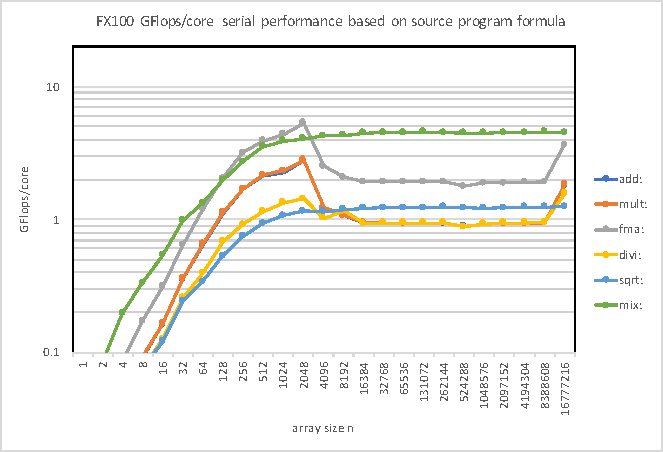
\includegraphics[width=0.45\textwidth]{figs/workload-user.pdf}
%	\caption{workload-user}
%	\label{fig:workload-user}
%	\end{figure}
\begin{figure}[tb]
%\begin{minipage}{0.49\hsize}
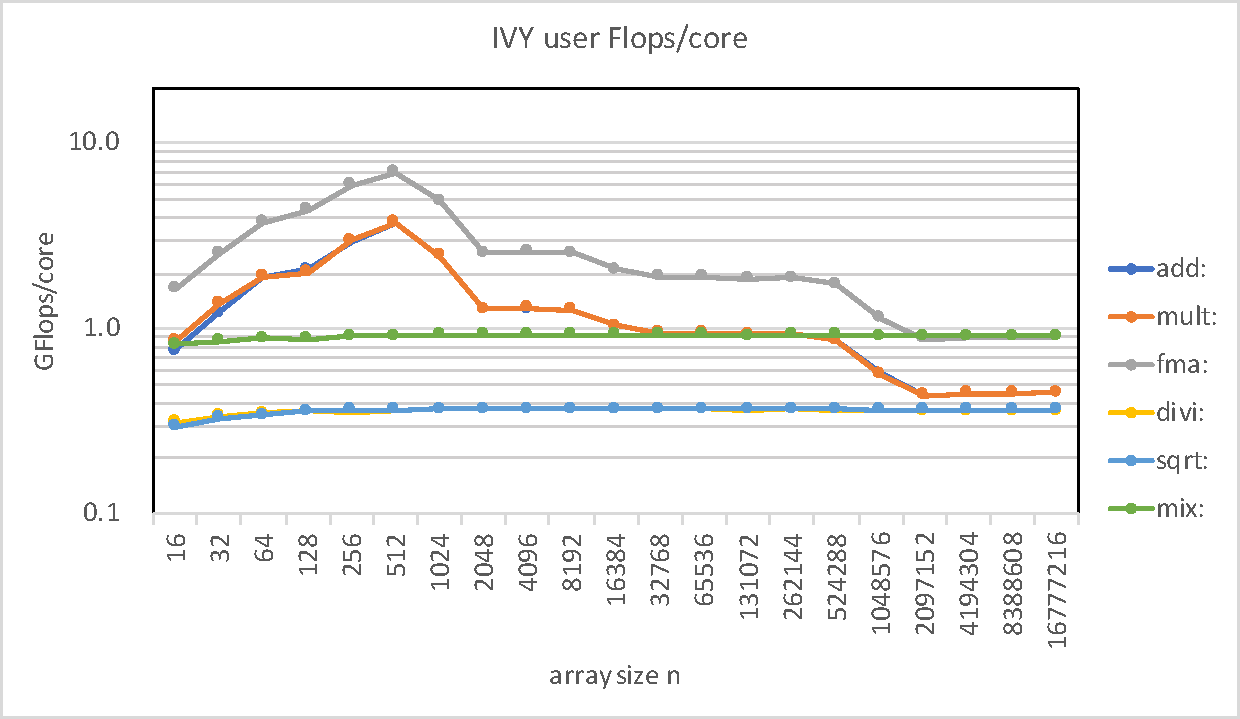
\includegraphics[width=0.5\textwidth]{figs/workload-ivy-user.pdf}
\caption{User perspective workload and performance}
\label{fig:workload-user}
\end{figure}
%\end{minipage}
\begin{figure}[tb]
%\begin{minipage}{0.49\hsize}
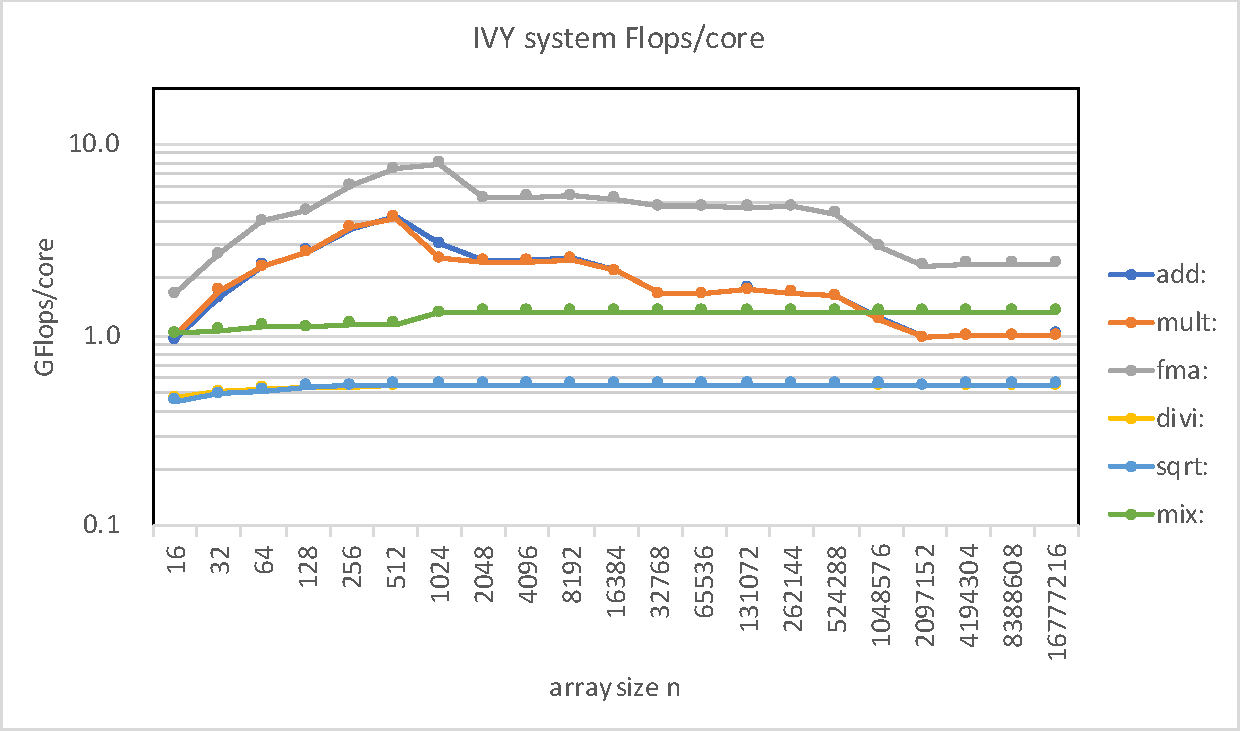
\includegraphics[width=0.5\textwidth]{figs/workload-ivy-system.pdf}
\caption{System perspective workload and performance}
\label{fig:workload-system}
%\end{minipage}
\end{figure}
%
\begin{figure}[tb]
%\begin{minipage}{0.49\hsize}
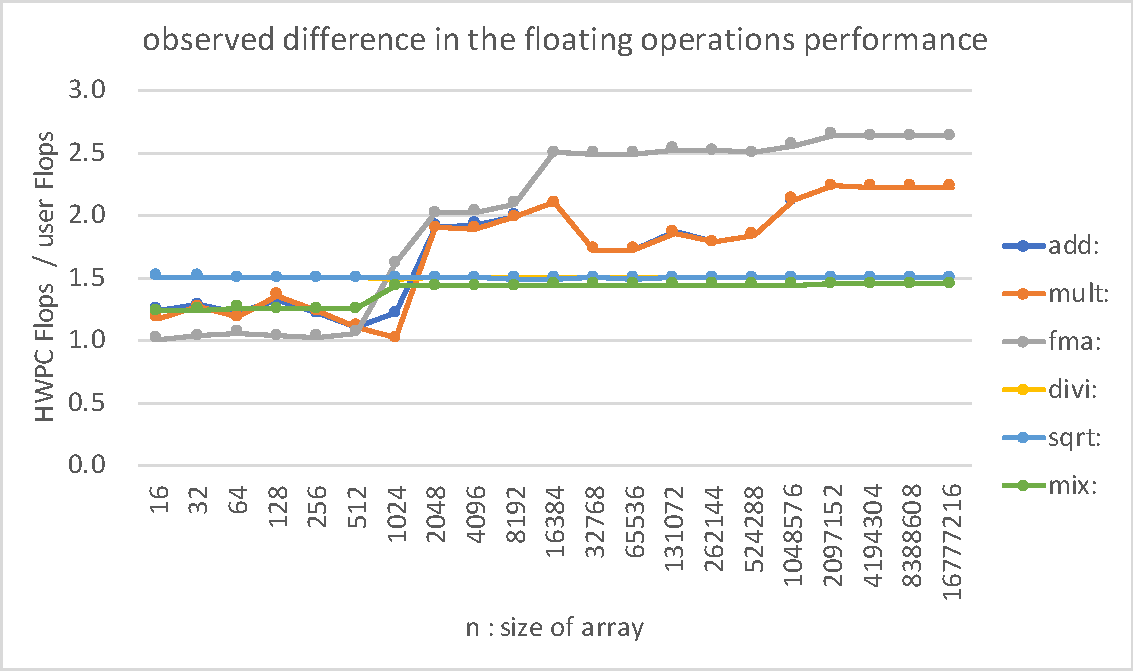
\includegraphics[width=0.5\textwidth]{figs/workload-ivy-difference.pdf}
\caption{Difference between the workloads}
\label{fig:workload-difference}
%\end{minipage}
\end{figure}

This simple example clearly indicates that the performance evaluation of
scientific applications on HPC systems must be associated with a clear
definition of workload. The example also suggests that if conditions allow, the evaluation should be
conducted for both user and system perspectives.
A detailed analysis of a similar example is given in section
\ref{subsection:basic-kernels}.

%%
\section{Performance Monitoring Library}
\label{section:PMlib}

%
\subsection {Overview of PMlib}
PMlib is an open source library for monitoring the performance of scientific applications
and is able to measure the listed types of workload discussed
in the previous
section, i.e. arithmetic, application, and HWPC workloads.
Users can insert start/stop API statements provided in the source code.
Each measurement section has minimal properties such as name, type of operation,
exclusiveness, and workload value.
The reports from PMlib is classified into threads, processes, and sections
depending on the controlling environment variable.

%
\subsection{PMlib API}
%\label{subsection:PMlib-API}
PMlib provides APIs for C++ and Fortran programs.
There is a limited number of APIs which must be called in most applications.
C++ APIs are shown in Table~\ref{tab:PMlib-API}. 
Equivalent Fortran APIs that follow similar naming convention as
$f\_pm\_${\footnotesize{C++API}} are also provided.

\begin{table}[htb]
\scriptsize
\caption{list of basic APIs provided by PMlib}
\label{tab:PMlib-API}
\footnotesize
\begin{tabular}{l|l|l} \hline
\scriptsize
C++	& function	&	arguments	\\ \hline \hline
initialize	& initial setup	& number of sections (optional)	\\ %\hline
setProperties	& set sections property	& label, type, exclusiveness \\ %\hline
start	& start of section	& label \\ %\hline
stop	& end of section	& label, arithmetic workload (optional)	\\ %\hline
print	& basic report	& filename, comments, sort order	\\ %\hline \hline
printDetail	& per process report	& filename, sort order	\\ %\hline
printThreads	& per thread report	& filename, sort order	\\ \hline
\end{tabular}
\end{table}

The following example shows a Fortran program calling PMlib.

%	\begin{lstlisting}[caption={using PMlib in Fortran program}]
\begin{lstlisting}
program main
call f_pm_initialize (Nsections)
call f_pm_setproperties ("section1",icalc,iexcl)
call f_pm_start ("section1")
call some_computation (fops)
call f_pm_stop ("section1",fops,ncall)
call f_pm_print ("",isort)
call f_pm_printdetail ("",ilegend,isort)
end
\end{lstlisting}

%
\subsection{Choosing workload type}
\label{subsection:Choosing-workload-type}

The choice of arithmetic workload or HWPC workload is made by a
run-time environment variable HWPC\_CHOOSER.
A possible choice of the HWPC\_CHOOSER value is:
\begin{quote}
\begin{small}
%	\begin{verbatim}
FLOPS\textbar BANDWIDTH\textbar VECTOR\textbar CACHE\textbar CYCLE%
\textbar user
%	\end{verbatim}
\end{small}
\end{quote}

If the arithmetic workload is measured,
The number of arithmetic operations or the formula defining the workload
must be provided to PMlib API as user argument.
PMlib accumulates the workload per section sandwiched by start and stop APIs.
In practice, counting the number of arithmetic operations in the application
source code can be a non-trivial task, and automating such a task is desirable.
%
If the application is written in Fortran,
we can utilize the related research~\cite{Hoshimoto:2015},~\cite{ccaebt:HPCAsia2018}
to let the parser program analyze the Fortran source code
and produce JSON intermediate reports showing the arithmetic operations counts.
Then, a second filter can be used to produce the partial Fortran source program
including call statements for PMlib API with provisioned arguments.
{\color{blue} Remark. This second filter is under development as of this paper.  }
Fig.~\ref{fig:ccaebt4PMlib} shows the schematic flow used to accomplish this process.

\begin{figure}[tb]
\centering
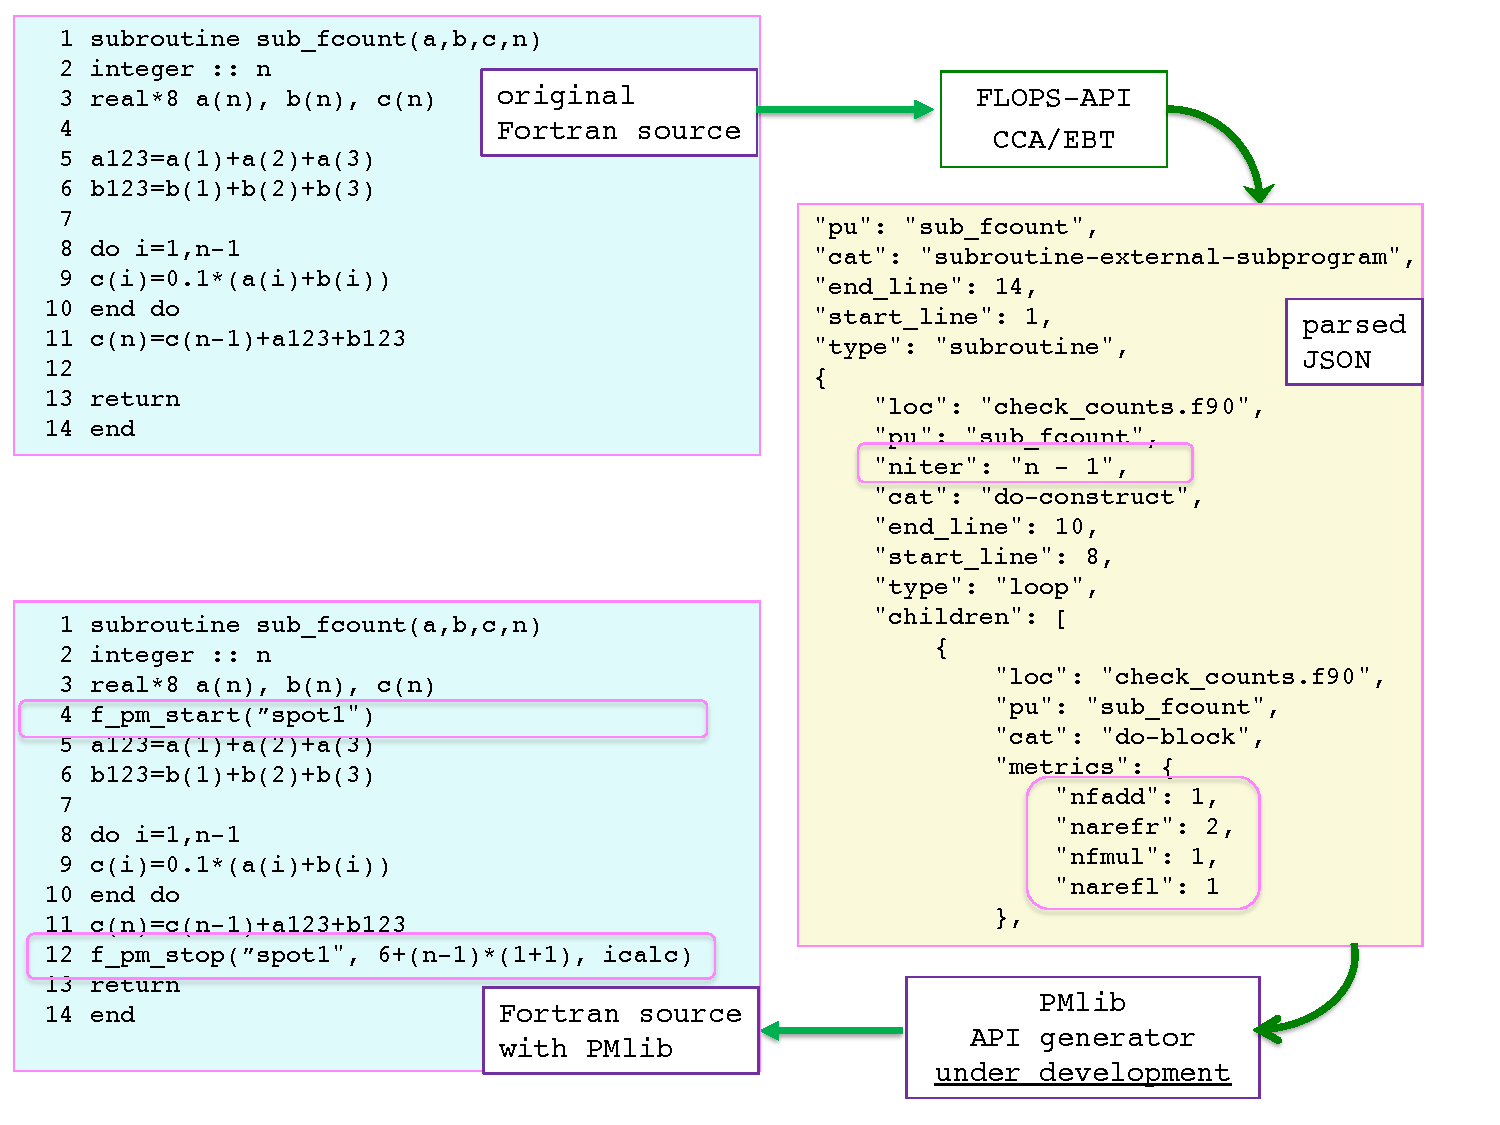
\includegraphics[width=0.5\textwidth]{figs/ccaebt4PMlib.pdf}
\caption{Counting the operation with ccaebt parser program}
\label{fig:ccaebt4PMlib}
\end{figure}

If the HWPC workload is measured,
PMlib automatically detects the type of hardware and reads the HWPC
event statistics at each of the start/stop API.
In the HWPC workload mode, PMlib does not utilize the user given argument value,
if any.
While PAPI has a good set of user APIs and is well documented,
it is not a simple task to choose the correct native event sets and masks
for specific target processor instructions, and to sort out the event
values for a desired performance category using a limited set of HWPC.
For example,
the standard output from the papi\_native\_avail command on a server with
an Intel Skylake Gold processor produces 5000+ lines.

PMlib facilitates the application developer's intent to
categorize raw performance information from HWPC, and to
help evaluate performance.
Once PMlib APIs are coded in the application, PMlib preserves the HWPC
portability. That is, PMlib chooses and reads the appropriate HWPC event
set, if the application runs on different HPC systems.

\subsection{High-resolution timer available to PMlib}
PMlib is a portable package that utilizes the Linux standard timer
{\tt gettimeofday} by default. It also has the installation option to utilize
a system specific high-resolution low overhead timer if such timer is
available on the platform.

Fig.~\ref{fig:precise-timer} shows a comparison of a standard timer and
the high-resolution timer on the two HPC systems highlighted in the
previous section.
PMlib has a provision to use them as an installation option.

\begin{figure}[tb]
\centering
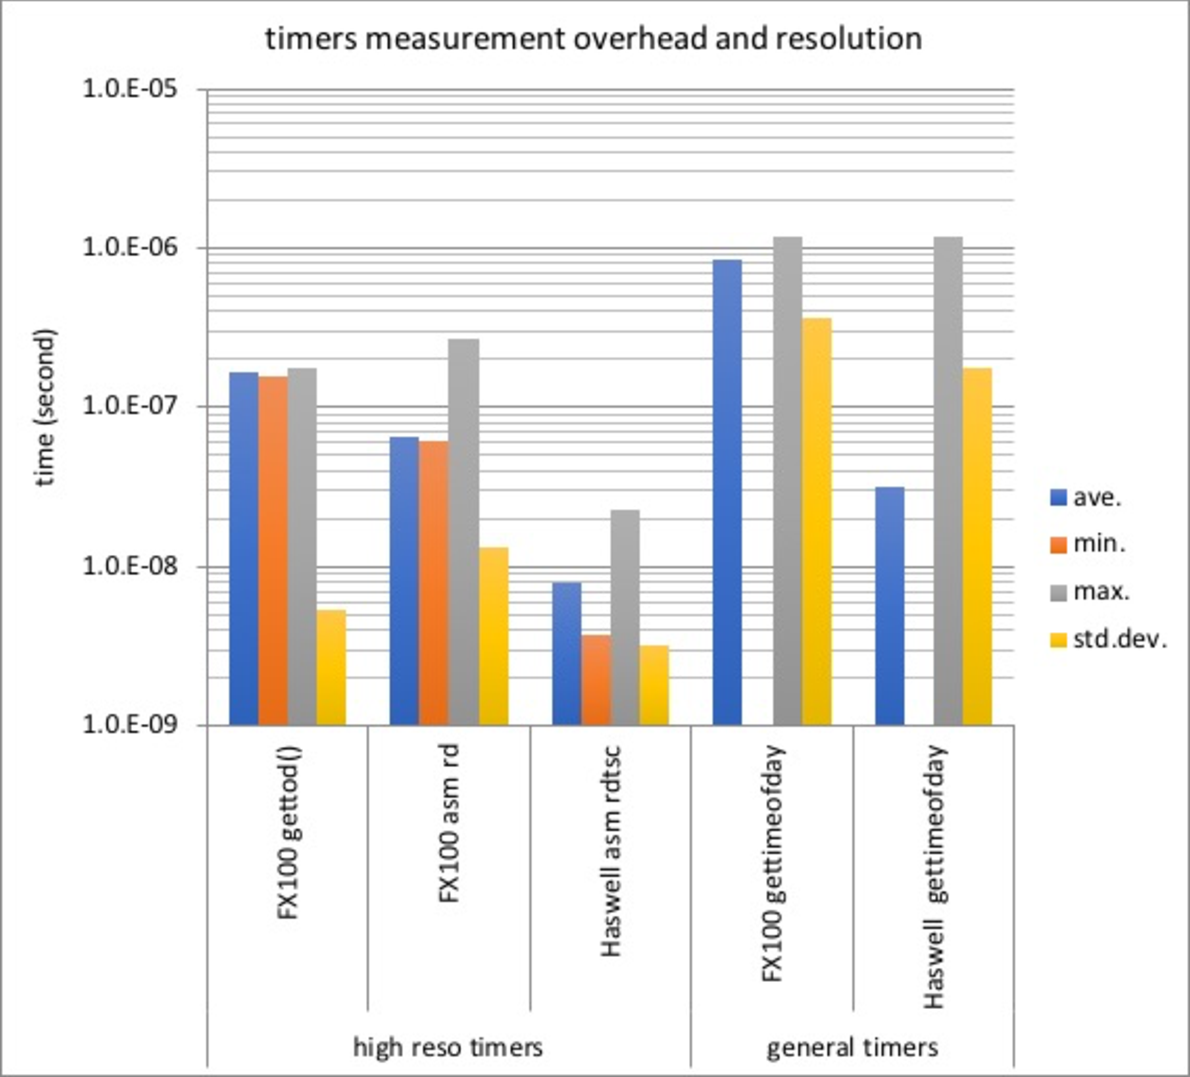
\includegraphics[width=0.45\textwidth]{figs/precise-timer.pdf}
\caption{general timer and precise timer}
\label{fig:precise-timer}
\end{figure}

\subsection{Output information}
\label{subsection:PMlib-output-information}
The default output information from PMlib is a blocked text report based on
the time-averaged performance statistics.
PMlib is also able to produce the
Open Trace Format (OTF)~\cite{Knupfer:2006},~\cite{OTF:webpage-public}
tracing files that may contain the shorter interval statistics for visualization.
%
%	In future papers, we may include TRAiL contents
%
%	Web browser visualization tool TRAiL~\cite{trail}~.%
%	\begin{figure}[tb]
%	\centering
%	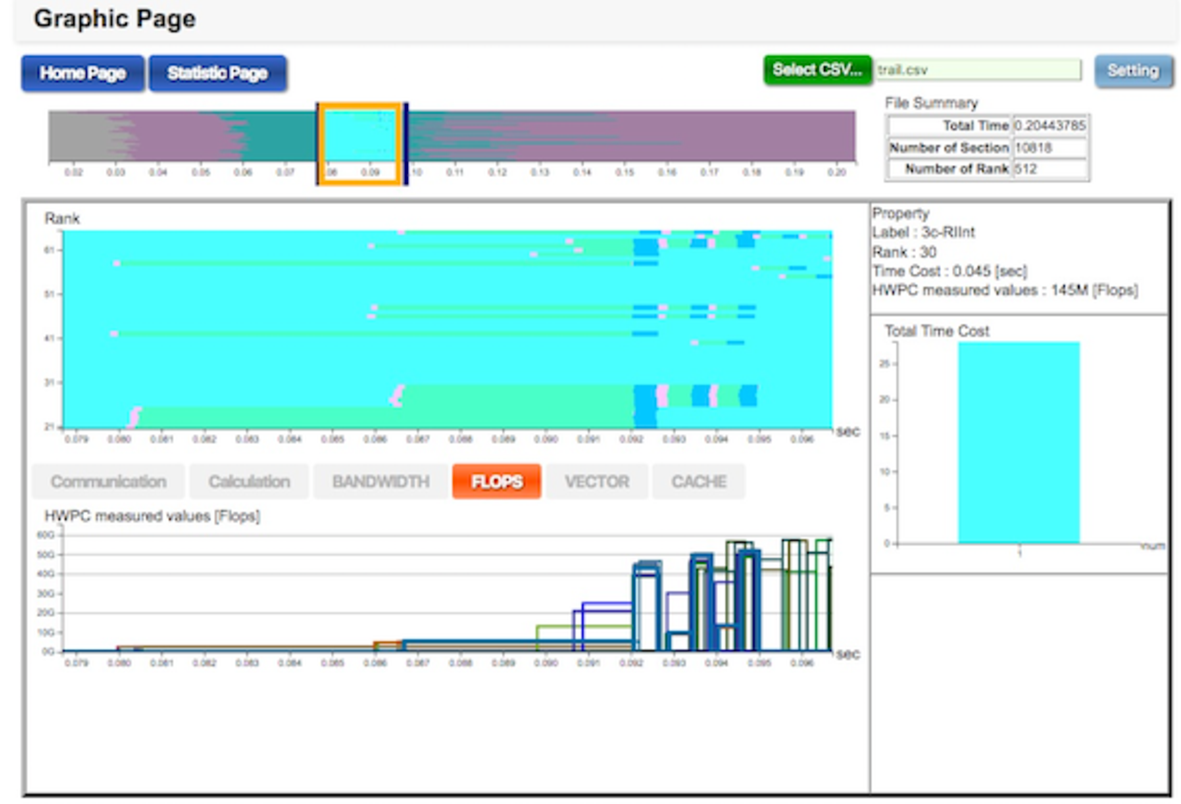
\includegraphics[width=0.45\textwidth]{figs/TRAiL-small.pdf}
%	\caption{tracing visualization using PMlib and TRAiL}
%	\label{fig:TRAiL}
%	\end{figure}


\subsection{Other performance evaluation tools and related research}
\label{subsection:related-research}
Numerous tools have been developed to evaluate the performance of HPC systems.
In general, open source tools are designed to be portable.
Their functionalities are distinct and in many cases, multiple tools
are used in sequence to obtain the desired performance information.
These tools are classified as either sampling or tracing tools and they each have different overheads.
Commercial vendor tools are used for many HPC systems.
They are best used for specific processor types.
HPC systems vendors also supply performance evaluation tools
that are native to their systems.
They are integrated into systems and are easy to use in general,
but availability is limited to only the vendor's HPC systems.

Some of the commonly used tools are listed below.
In the open source category:
\begin{itemize}
	\item Scalasca \cite{Scalasca:2017},\cite{Scalasca:2010}
			: trace generation, Score-P infrastructure
	\item Extrae \cite{Extrae:webpage} :  trace generation
	\item PAPI \cite{PAPI:5.6} : API to access HWPC
	\item Linux perf tools : API to access HWPC
\end{itemize}
In the commercial vendor category:
\begin{itemize}
		\item Intel VTune \cite{Intel:VTune} : Intel processors
		\item PGI Profiler \cite{PGI:Profiler} : X86 and GPU
\end{itemize}
these existing tools all utilize the processor performance information
based on HWPC workload, i.e. system workload.
PMlib appears to be the only tool that enables arithmetic and/or application
workload evaluation.

%%
\section{Performance evaluation using PMlib}
\label{section:using-PMlib}

Some examples that involve the use of PMlib for performance evaluation are shown in this
section.
The list of servers used for the measurements are shown below.
\begin{itemize}
{
%	\setlength{\itemsep}{-5pt}
%	\setlength{\topsep}{2mm}
\item SGI Intel Ivybridge server
\item SGI Intel Skylake server
\item Fujitsu prime HPC FX100
}
\end{itemize}
Their processor specifications and the major performance specifications
are listed in Table~\ref{tab:server-config}.

\newif\ifTwoservers
\newif\ifThreeservers
\Twoserversfalse
\Threeserverstrue
%\tiny
%\footnotesize
%\small
\begin{table}[tb]
\scriptsize
\caption{server configuration and hardware specification}
\label{tab:server-config}
\footnotesize

\ifTwoservers
\begin{tabular}{l|c|c} \hline
\scriptsize
system			&	FX100	&	Skylake	\\ \hline
CPU				&	SPARC64 XIfx	&	Gold 6148	\\ \hline
core GHz		&	1.975	&	2.4	\\ \hline
core Gflops	&	31.6	&	〜30	\\ \hline
L1\$ size (D,I)		&	64KB, 64KB	&	32KB, 32KB	\\ \hline
L1D\$ BW GB/s	&	140/R+70/W	&	154/R + 77/W	\\ \hline
\$ Linesize 	&	256B	&	64B	\\ \hline
L2\$ size		&	-	&	1MB	\\ \hline
L2\$ BW GB/s/core	&	-	&	154 ( ~70)	\\ \hline
LL\$ size		&	12MB	&	28MB(1.4MB/c)	\\ \hline
LL\$ BW GB/s/core	&	70/R+35/W	&	77 ( ~43)	\\ \hline
Memory			&	HMC(8x16Ls)	&	DDR4-2666	\\ \hline
Mem GB/s/[CMGcpu]	&	120/R+120/W	&	128	\\ \hline
\#cores/[CMGcpu]	&	16	&	20	\\ \hline
\end{tabular}
\fi

\ifThreeservers
\begin{tabular}{l|c|c|c} \hline
\scriptsize
Symbol			&	FX100	&	SKY		&	IVY \\ \hline
Platform		&	FX100	&	Skylake & Ivybridge\\ \hline
CPU				&	SPARC64 XIfx	&	Gold 6148	&	E5-4620v2	\\ \hline
core GHz		&	1.975	&	2.4	&	2.6 \\ \hline
core Gflops	&	31.6	&	~30	\\ \hline
\#core/cpu*	&	16	&	20	&	8	\\ \hline
L1\$ size(D,I)		&	64KB, 64KB	&	32KB, 32KB	\\ \hline
L1D\$ BW GB/s	&	140/R+70/W	&	154/R + 77/W	\\ \hline
\$ Linesize 	&	256B	&	64B	&	64B	\\ \hline
L2\$ size		&	-	&	1MB	&	256KB	\\ \hline
L2\$ BW GB/s/c	&	-	&	154 ( ~70)	\\ \hline
LL\$ size		&	12MB	&	28MB	&	20 MB	\\ \hline
LL\$ BW GB/s/c	&	70/R+35/W	&	77 ( ~43)	\\ \hline
Memory			&	HMC(8x16Ls)	&	DDR4-2666	& DDR3-1600	\\ \hline
Mem GB/s/cpu*	&	120/R+120/W	&	128	\\ \hline
\#cores/cpu*	&	16	&	20	\\ \hline
\multicolumn{4}{l}{\scriptsize\hspace{5mm} remark. cpu* indicates processor or
CMG }\\
\end{tabular}
\fi

\end{table}

%
\subsection{Basic kernels}
\label{subsection:basic-kernels}

The basic kernels which are composed of four basic arithmetic operations in addition to the square root operation
are evaluated first.
The Fortran source program for measuring kernels is shown in List 1.

\begin{lstlisting}[caption={basic kernels (partial list)}]
subroutine sub_add(a,b,c,n)
do i=1,n
c(i)=a(i)+b(i)
end do

subroutine sub_mult(a,b,c,n)
do i=1,n
c(i)=a(i)+b(i)
end do

subroutine sub_fma(a,b,c,n)
d=real(n)
do i=1,n
c(i)=a(i)+b(i)*d
end do

subroutine sub_divide(a,b,c,n)
do i=1,n
c(i)=b(i)/a(i)
end do

subroutine sub_sqrt(a,b,c,n)
do i=1,n
c(i)=sqrt(a(i))
end do

subroutine sub_mix(a,b,c,n)
do i=1,n
c(i)=1.0/sqrt(a(i)**2+b(i)**2)
end do
\end{lstlisting}

These basic kernels are computed as single-strided loops without dependencies.
%	They are expected to be efficiently processed by exploiting
%	parallel execution pipelines and wide units.
A compile option to assign double precision to real variables is enabled,
and automatic parallelization is disabled.
So the kernels are simply vectorized as wide SIMD instructions and
executed on execution pipelines on the measuring systems.
The terms vectorization and SIMD are used synonymously hereafter.

\subsection{Kernel performance on FX100 in long loops}
\label{subsection:long-kernels-fx100}
%
% We must cut the following important remarks because of the short space.
%
The computing time of these kernels is measured on FX100 system
for several iterations.
After subtracting the calling overhead time,
the average computing time for each kernel is obtained.
Note that the do loop cost is included in the average computing time.
%
%
\if 0
Typical HPC systems are simultaneously shared by many users and tend to
suffer from perturbation influences called noise caused by other processes,
shared file systems, networks with shared topology, etc.
This influence is usually more than that of a small dedicated system.
It is not an easy task to eliminate this noise even for simple measurements 
when measuring small granularity computation time.
On the user side, noise elimination can be addressed via statistical
approaches. These include the addition of an outer loop for repeated
measurement and the filtering of measurements values that fall outside of
a standard deviation window.
\fi
%
%
Fig.~\ref{fig:fx100-gflops-user-long-R8} shows the 
performance of the basic kernels based on the arithmetic workload,
i.e. user performance,
measured on an FX100 system using the loop length of
\begin{math}
n=1,2,4,..,2^{24}
\end{math}
.
%	the noise has been removed as indicated above.
Fig.~\ref{fig:fx100-gflops-system-long-R8} shows the 
performance based on the system workload, i.e. system performance.

%	revert for double blind
\begin{figure}[b]
%	\begin{figure}[tb]
\centering
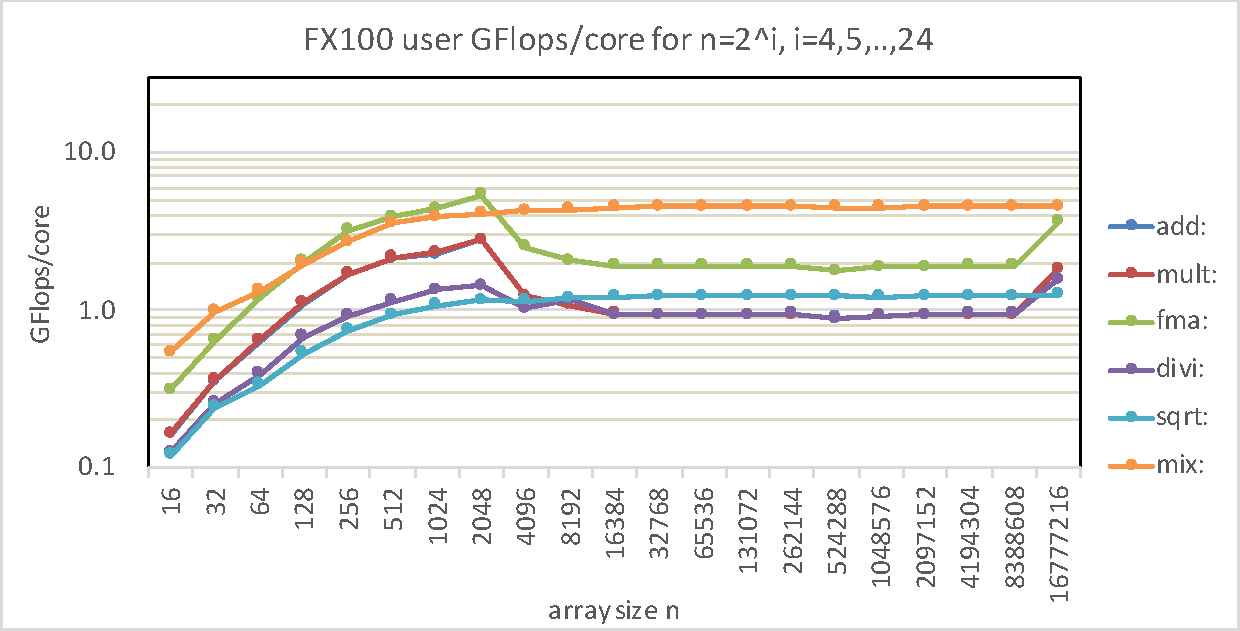
\includegraphics[width=0.45\textwidth]{figs/fx100-gflops-user-long-R8.pdf}
\caption{user performance of FX100 for basic kernels}
\label{fig:fx100-gflops-user-long-R8}
\end{figure}

\begin{figure}[tb]
\centering
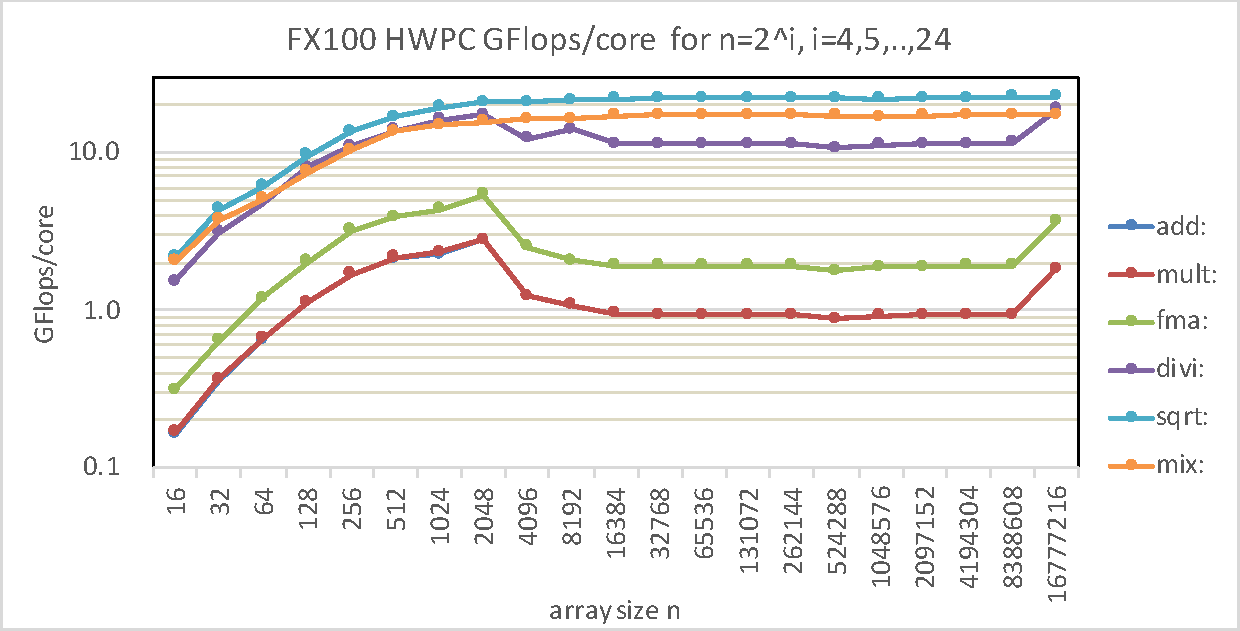
\includegraphics[width=0.45\textwidth]{figs/fx100-gflops-system-long-R8.pdf}
\caption{system performance of FX100 for basic kernels}
\label{fig:fx100-gflops-system-long-R8}
\end{figure}

\begin{figure}[tb]
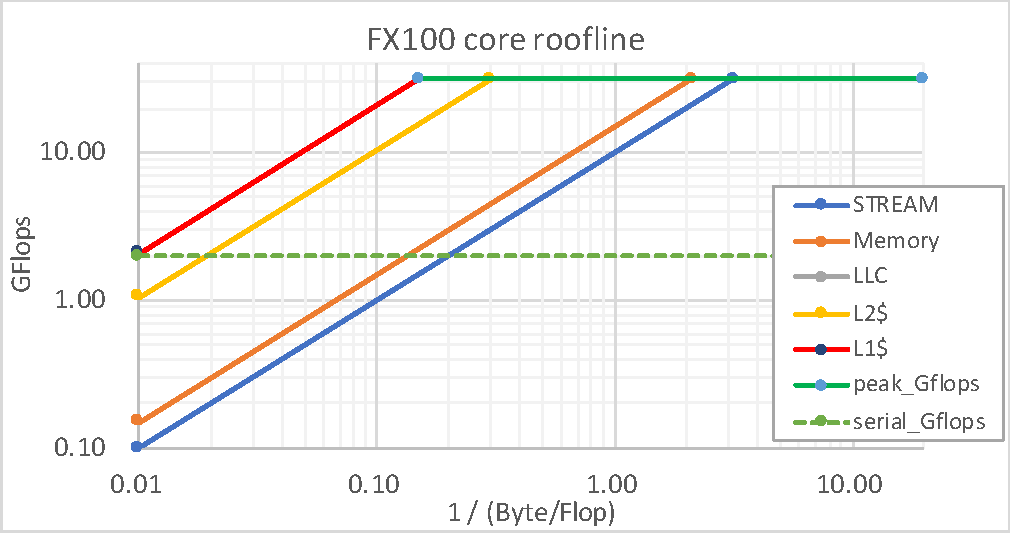
\includegraphics[width=0.45\textwidth]{figs/roofline-fx100.pdf}
\caption{roofline envelop of FX100}
\label{fig:roofline-fx100}
\end{figure}

In both of these figures,
the performance of add/mult/fma tends to improve with an increase of
the loop length until the L1 cache size limit is reached,
and subsequently drops to the bandwidth constrained performance level
of the next level cache.
This performance tendency for add/mult/fma is consistent with the reports
from other related research investigations.
It can be associated with the
the roofline~\cite{Williams:2009}
envelop which is shown in Fig.~\ref{fig:roofline-fx100}

The performance of div/sqrt/mix shows quite different tendency, and
Their system performance stays much higher than the user performance.

PMlib HWPC report for this case is shown in Table~\ref{tab:PMlib-report-HWPC}.
Native HWPC events are sorted according to the choice of the
environment variable HWPC\_CHOOSER=VECTOR as explained in
\ref{subsection:Choosing-workload-type} for user evaluation.
According to the report,
the number of required operations for division is almost an order of magnitude
larger than that for addition, even though their arithmetic workload
is the same.
Compiler optimization transforms
a division arithmetic statement into a series of reciprocal
approximation and multiply-add instructions, rather than issuing
a simple division instruction. They takes advantage of
data width of SIMD instruction and maintain high flop/byte ratio.
So the apparent HWPC performance of this operation becomes very high,
but the user perspective performance is much lower, almost the same as
add/mult in this case. In fact, divide kernel runs much slower than add/mult,
if not vectorized at all.
The comparison of system/user performance ratio is shown in
Table~\ref{tab:ratio-system-user-fx100}. The numbers in the table can be
directly obtained from HWPC\_CHOOSER=FLOPS setting.
%	This causes the difference between 
%	Figure~\ref{fig:fx100-gflops-user-long-R8}
%	and
%	Figure~\ref{fig:fx100-gflops-system-long-R8}
%	.
Without having to read the assembly code generated by the compiler,
users can capture some idea from the statistics of PMlib HWPC report.
\begin{table}[b]
%	\begin{center}
%	\scriptsize
\centering
\caption{PMlib HWPC report(edited)}
\label{tab:PMlib-report-HWPC}
\footnotesize
\input{figs/stdout.PMlib-report-HWPC.txt}
%	\end{center}
\end{table}

The reason for div/sqrt/mix performance curves not having the drop near
the L1 cache size limit is explained by the high computational density.
\begin{table}[b]
%	\scriptsize
%	\begin{center}
\centering
\caption{ratio of system/user performance of FX100 for basic kernels}
\label{tab:ratio-system-user-fx100}
%	\footnotesize
\begin{tabular}{l|c|c|c|c|c|c} \hline
%	\scriptsize
type &	add	&	mult &	fma &	div &	sqrt &	mix \\ \hline
ratio &	1.0 &	1.0 &	1.0 &	12.0 &	18.0 &	38.0 \\ \hline 	
\end{tabular}
%	\end{center}
\end{table}


\subsection{Kernel performance on FX100 in short loops}
\label{subsection:short-kernels-fx100}

In the short loop region,
the overhead to process loop set-up and update cannot be neglected,
and this performance is associated with data access latency.

FX100 has SIMD 256 bit wide arithmetic and data access instructions.
Its floating point operations can be sorted in width as represented below.
\begin{quote}
\begin{small}
\begin{verbatim}
fpdp1  : "1FLOPS_INSTRUCTIONS";
fpdp2  : "2FLOPS_INSTRUCTIONS";
fpdp4  : "4FLOPS_INSTRUCTIONS";
fpdp8  : "8FLOPS_INSTRUCTIONS";
fpdp16 : "16FLOPS_INSTRUCTIONS";
\end{verbatim}
\end{small}
\end{quote}
The floating point operation workload including single precision
and double precision data types is given as:
\begin{align}
	\mathrm{W}_{hwpc} & = \mathrm{fpdp1} + 2.0*\mathrm{fpdp2} + 4.0*\mathrm{fpdp4} \nonumber \\
			& + 8.0*\mathrm{fpdp8} + 16.0*\mathrm{fpdp1} 
\end{align}

Fig.~\ref{fig:fx100-gflops-short-R8}
shows the close-up performance characteristics of the same kernels for
\begin{math}
n=1,2,3,..,50
\end{math}
.
The close-up curves do not show the gradual increase. Instead, they
show the steep stepping shapes at multiples of a constant interval.
This is a common observation for systems with processors that support SIMD,
and the interval corresponds to the data width of the SIMD instructions.
For example, FX100 double precision (64 bits) arithmetic can utilize
256 bit instructions, and the resulting interval is
\begin{math}
256 / 64 = 4
\end{math}
.
So the performance is the best at 4n, then 4n+1, followed by 4n+2,
and lowest at 4n+3.
Fig.~\ref{fig:fx100-gflops-short-R8} highlights the fact that
program coding practices that maintain the loop length as a multiple of
the SIMD width has a significant impact, especially for short loop computation.
For single precision (32 bits), the interval becomes
\begin{math}
256 / 32 = 8
\end{math}
, and the performance impact is even stronger as seen in
Fig.~\ref{fig:fx100-gflops-short-R4} for FX100.

\begin{figure}[tb]
\centering
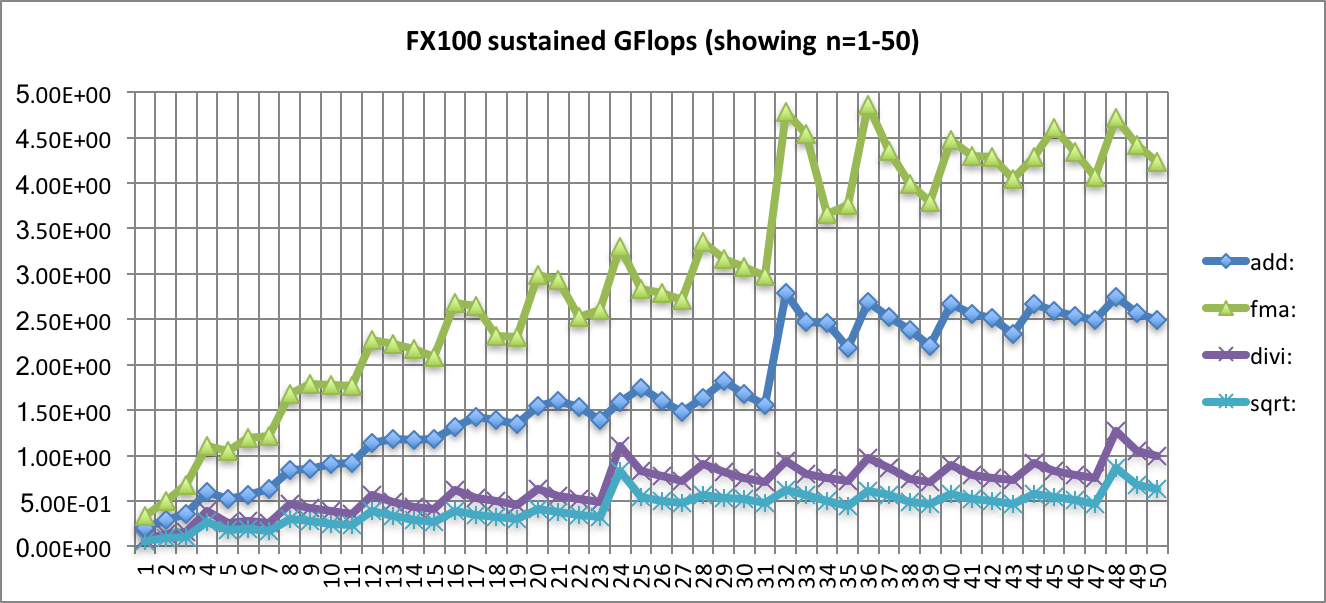
\includegraphics[width=0.45\textwidth]{figs/fx100-gflops-short-R8.pdf}
\caption{FX100 performance close up}
\label{fig:fx100-gflops-short-R8}
\end{figure}

\begin{figure}[tb]
\centering
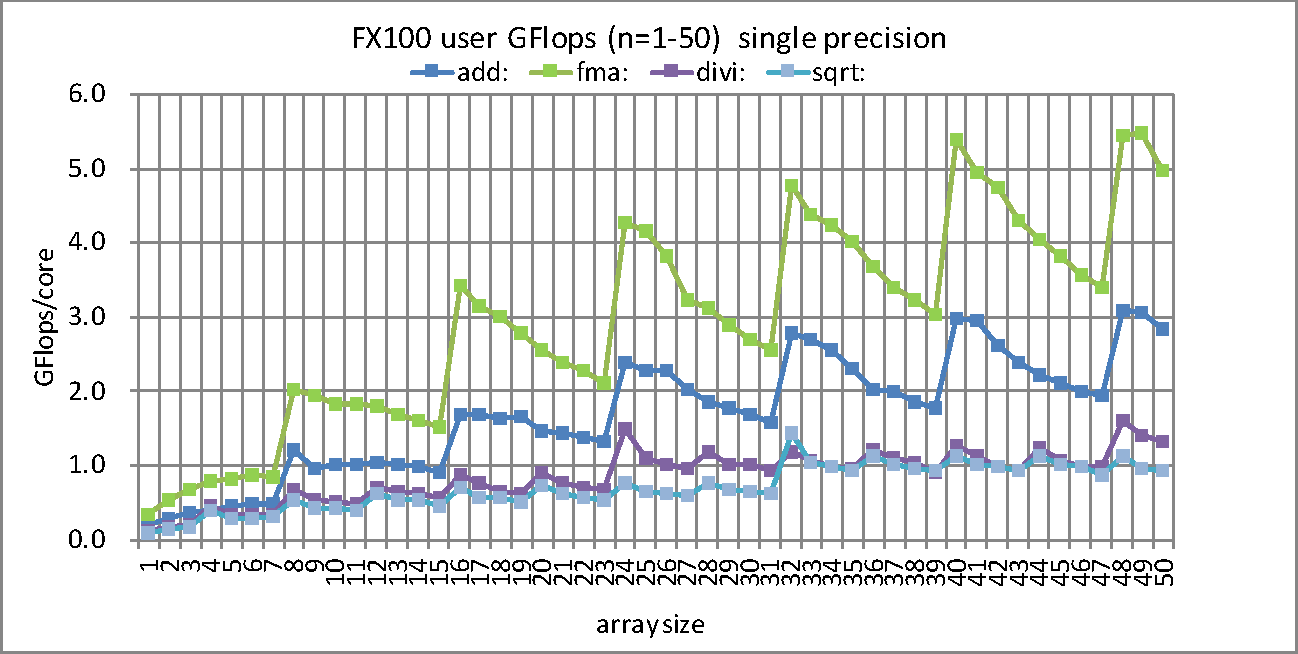
\includegraphics[width=0.45\textwidth]{figs/fx100-gflops-short-R4.pdf}
\caption{FX100 performance close up for single precision kernels}
\label{fig:fx100-gflops-short-R4}
\end{figure}

IVY also shows the similar performance characteristics.
Fig.~\ref{fig:ivy-gflops-short-R8} shows the user performance
of the same basic kernels on IVY. The stepping behavior of SIMD on IVY
appears to be less than that of FX100.
\begin{figure}[tb]
\centering
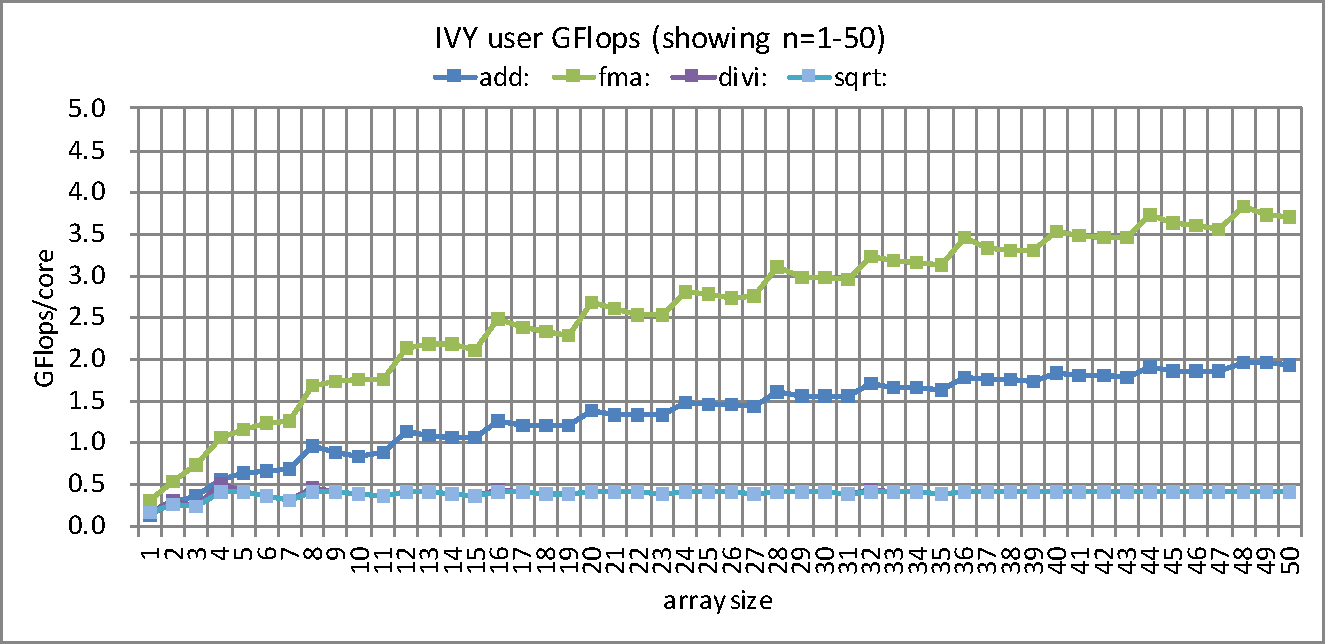
\includegraphics[width=0.45\textwidth]{figs/ivy-gflops-short-R8.pdf}
\caption{user performance of IVY for basic kernels}
\label{fig:ivy-gflops-short-R8}
\end{figure}

These examples demonstrate the usefulness of PMlib user mode
and HPWC mode measurements in understanding the performance
within a program block of interest.

%
% No space. STREAM subsection is omitted.
%
\if 0
\subsection{STREAM}
\label{subsection:STREAM}
STREAM benchmark~\cite{stream:1995}
has been widely used to measure the memory bandwidth of computer systems.
The standard output of this benchmark includes information on the
basic arithmetic performance of copy, multiplication, addition,
and multiplication\&addition, i.e. arithmetic workload perspective.

STREAM HWPC performance shows different characteristics compared to
the reported STREAM arithmetic performance. Their performance is influenced by
the combined effect of compilers and their optimization options.
Although this paper does not intend to provide an exhaustive review of this process,
a few points of interest related to the bandwidth are presented.

The STREAM Fortran OpenMP result for IVY using 8 threads packed in a CPU
is shown first in Fig.~\ref{fig:stream-ivy-1cpux8T}.
Then, we compare fig.\ref{fig:stream-ivy-1cpux8T}
with
Fig.~\ref{fig:stream-ivy-4cpux2T}, 
which shows the result using 8 threads scattered over 4 CPUs.

The values reported by STREAM for packed thread assignment is better
if the streaming-store option is used.
%
%	% minipage
%	\begin{figure}[tb]
%	\begin{minipage}{0.48\hsize}
%	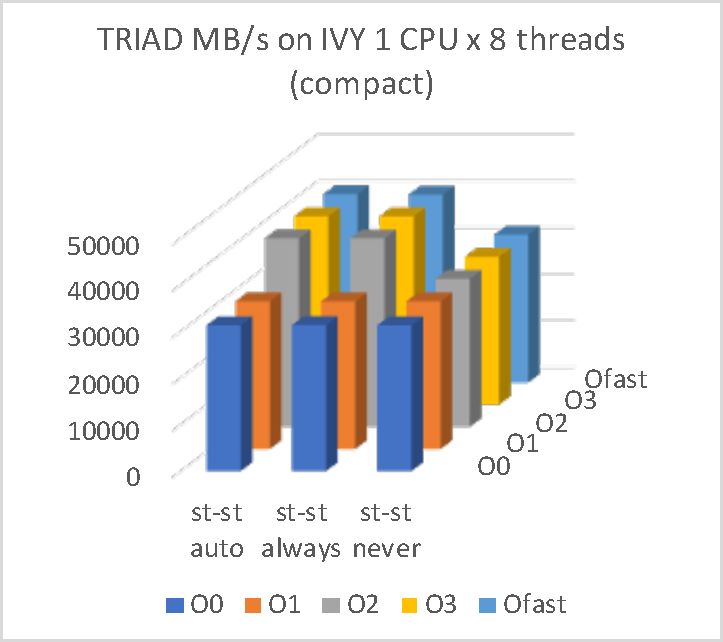
\includegraphics[width=0.98\textwidth]{figs/stream-ivy-1cpux8T.pdf}
%	\caption{stream-ivy-1cpux8T}
%	\label{fig:stream-ivy-1cpux8T}
%	\end{minipage}
%	\begin{minipage}{0.48\hsize}
%	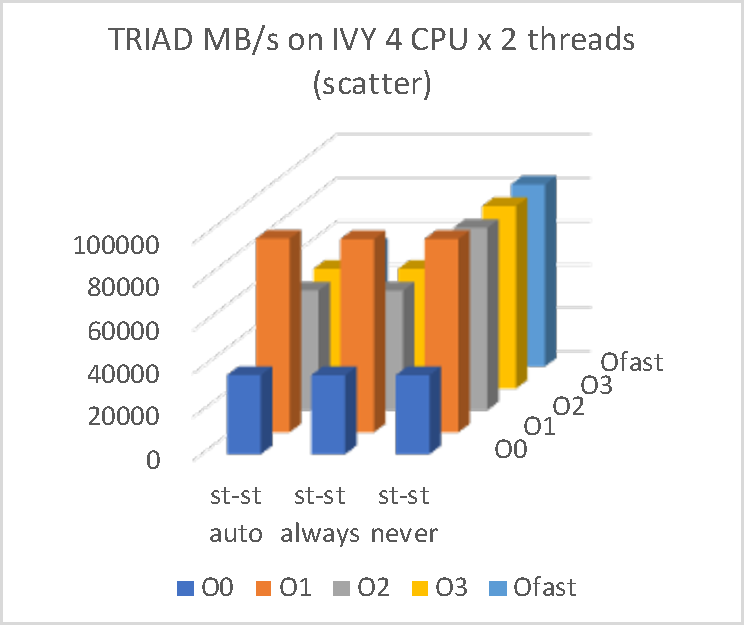
\includegraphics[width=0.98\textwidth]{figs/stream-ivy-4cpux2T.pdf}
%	\caption{stream-ivy-4cpux2T}
%	\label{fig:stream-ivy-4cpux2T}
%	\end{minipage}
%	\end{figure}
%
\begin{figure}[tb]
\centering
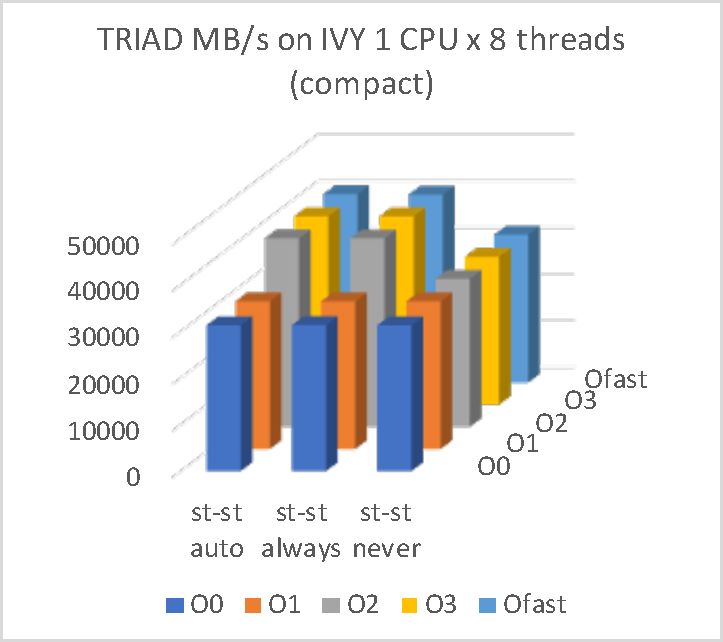
\includegraphics[width=0.45\textwidth]{figs/stream-ivy-1cpux8T.pdf}
\caption{Stream-ivy-1cpux8T}
\label{fig:stream-ivy-1cpux8T}
\end{figure}
\begin{figure}[tb]
\centering
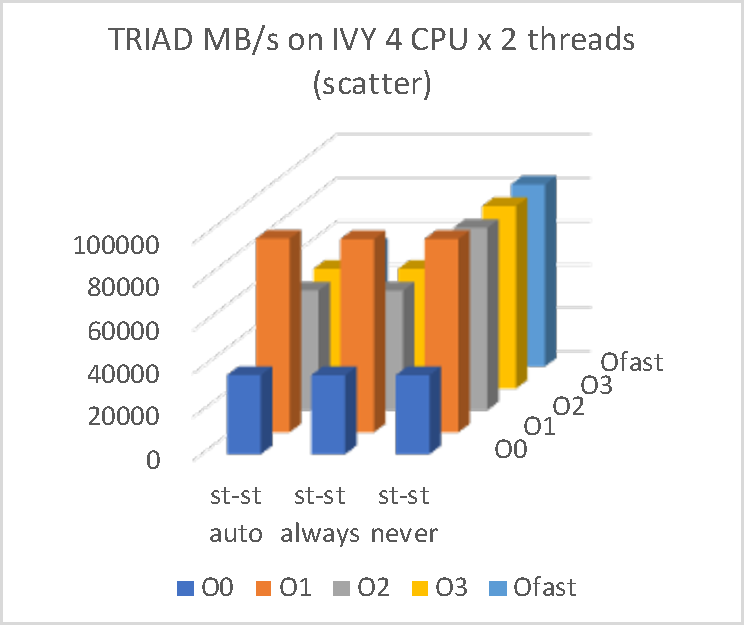
\includegraphics[width=0.45\textwidth]{figs/stream-ivy-4cpux2T.pdf}
\caption{Stream-ivy-4cpux2T}
\label{fig:stream-ivy-4cpux2T}
\end{figure}
\fi
%
%%
\section{Conclusion}
In this paper, we discussed the importance of multi-perspective evaluation
to understand the difference between the arithmetic workload coded as
the source program and the system workload executed as machine instructions,
which explains the gap between the performance
expected by users and the actually achieved performance on HPC systems.
We presented an open source library called PMlib, which analyzes the behavior
of these workloads.
PMlib provides an avenue for reporting the arithmetic/application workload
that is manually counted from a source code, as well as the actually executed
system workload.
It also provides detailed utilization reports of processor-specific hardware
including the categorized SIMD instruction statistics, the layered cache
hit/miss rate, and the effective memory bandwidth,
which are captured via hardware performance counters through PAPI library.
We could clarify the distinctive behavior by applying the PMlib to a target
program on different hardware architectures, and also verified that PMlib
allows users to conduct synthetic analyses of application performance,
thus enabling the users to obtain useful feedback for further optimizations
and better performance.

\section*{Acknowledgment}
This research used some computational resources of the K computer at the RIKEN Center for Computational Science in Kobe, Japan, and was carried out using the computer resources offered under the category of a general project by the Research Institute for Information Technology, Kyushu University.
%	\section*{References}
\bibliographystyle{jplain}
\bibliography{PMlib}
\end{document}

